\documentclass[a4paper, 11pt]{article}
\usepackage[utf8]{inputenc} % Change according your file encoding
\usepackage[margin=1in]{geometry}
\usepackage{graphicx}
\usepackage{caption}
\usepackage{subcaption}
\usepackage{float}
\usepackage[catalan,english]{babel}


%% Estil de Paràgraf
\setlength{\parskip}{4mm}
\setlength{\parindent}{0mm}

%% Estil lletra
\renewcommand{\familydefault}{\sfdefault}

\title{Activitat 7 - Web 2.0/25M}
\author{Ismael Peral Álvarez, Ferran Arau Castell}
\date{\today}

\begin{document}

\maketitle

\section{Introducció}

El projecte consisteix en dissenyar i arquitecturar la infraestructura necesària per allotjar una aplicació web. Concretament es tracta d'una aplicació intensiva en imatges que ha de servir a centenars d'usuaris i ha de estar disponible 24 hores al dia, 7 dies a la setmana.

El pressupost disponible és de 25 millons d'euros, amb els quals caldrà assumir els costos Capex i Opex. En conseqüència, cal provisionar els servidors de l'aplicació, els equips de xarxa i les cabines de discs. Cal assumir el cost dels serveis de housing, backup, xarxa i electricitat. Possiblement al llarg del projecte es modifiquin alguns d'aquests punts, segons les decisions que es prenguin.

La aplicació web amb la que es treballarà requerirà un model de tràfic vertical entre la plataforma i internet. Principalment amb un ample de banda de pujada de dades molt significatiu. És per aquest motiu, cal fer un esforç econòmic important en les prestacions de la xarxa.


\section{Requisits}

Els requisits mostren que cal disposar d'una infraestructura en alta disponibilitat i amb capacitat de creixement, és a dir, una infraestructura escalable horitzontalment. També s'estableix una SLA; cal garantir un temps de resposta inferior o igual a 100ms per petició HTTP.

Per poder complir els requisits cal desenvolupar una sèrie d'assumpcions, les quals es tractarà que siguin el més realistes possible. En primer lloc, cada petició tindrà un tamany mig de 600 bytes i cada resposta serà en mitjana de 180 KBytes. Cada petició generarà 5 accessos a disc d'un KByte cadascuna.

En quan a l'arquitectura, s'assumirà que l'aplicació no tindrà una capa de Base de Dades. No obstant, sí disposarà d'una capa d'aplicació on s'executarà el codi dinàmic d'aquesta. En l'apartat d'especificació de l'arquitectura es definirà una capa de caching, doncs caldrà assumir el percentatge d'encerts d'aquesta, entre d'altres.


\section{Arquitectura de sistemes}

A continuació s'exposa la arquitectura de la plataforma. S'ha tingut en especial consideració l'escalabilitat i l'alta disponibilitat de l'aplicació. És per això que la plataforma consta de diferents nivells desacoblats. Cadascun d'ells ha de funcionar segons els paradigmes de la orientació a serveis en sistemes distribuits, és a dir, cada nivell disposarà de la capacitat d'estar funcionant permanentment i d'escalar de manera independent segons les necessitats. 
També permet minimitzar l'aparició d'elements que puguin esdevenir un "Single Point of Failure". És a dir, elements que en el cas de fallar, tota la plataforma deixaria de donar servei. Finalment, s’aconsegueix detectar i pal·liar colls d'ampolla.

\begin{figure}[H]
    \centering
    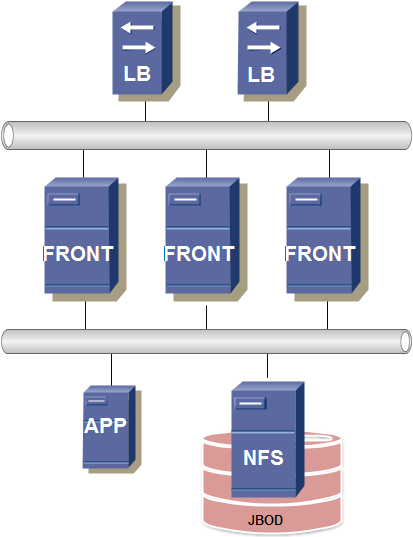
\includegraphics[width=1.0\textwidth]{IM}
    \caption{Arquitectura \label{fig:centralized}}    
\end{figure}

S'exposaran en primer lloc les capes que es trobin més a prop del client i s'anirà aprofundint.

En primer lloc, hi ha la capa de balanceig de càrrega o "proxy invers". Aquestes màquines rebran peticions web directament dels clients i les enrutaran cap el següent nivell. Tindran la finalitat de prendre la decissió de quina màquina rebrà la petició web. També seran terminadors SSL; actuaran de firewalls, doncs només enrutaran el tràfic per ports (de nivell 4) legítims, i seran la capa visible de la aplicació a internet.

En segon lloc, hi haurà la capa de "Frontals Web". Aquestes màquines tindran la capacitat de processar la petició web i enrutar aquelles parts que depenguin de codi dinàmic cap a la següent capa. Un cop la següent capa retorni els resultats tindran la capacitat de formatar la presentació de la resposta HTTP. D'altre banda, i com a punt més important, disposaran de gran part del contingut estàtic de l'aplicació. Donat que hi haurà volums molt grans de binaris, s'ha obtat perquè aquesta capa actuï com a cache de disc de les imatges de l'aplicació i del codi estàtic que s'executa al client. Les opciones inicials eren, o bé disposar d'un sistema d'emmagatzematge centralitzat amb totes les imatges o que tots els nodes de la capa disposesin de tots els fitxers estàtics. Donat que es va creure que ambdues eren solucions amb inconvenients insalvables per costos econòmics o per problemes de concurrència, es va optar per la solució de disposar d'alguns fitxers a cada node maximitzant aquells fitxers que més s'utilitzin.
Amb aquesta decisió s'aconsegueix minimitzar l'espai de disc de les màquines d'aquesta capa, però sense perdre rendiment en quan a latències de xarxa. Val a dir, que permetrà paral·lelitzar l'ample de banda de la xarxa a l'hora d'accedir a les imatges i no saturar la capa d'emmagatzematge. A més a més, permet que l'aplicació escali en capacitat d'usuaris de manera relativament senzilla. Evidentment fins a límits marcats per l'ample de banda de la xarxa de sortida a internet.   

A continuació, hi haurà la capa d'aplicació. Es tracte de nodes que executaran aquelles parts de codi necessaries per desenvolupar la lògica de negoci de l'aplicació. Serà una capa que no tindrà un pes molt important perquè es tracta d'una aplicació amb un ús intensiu en contingut estàtic. No obstant, val a dir que es tractaria d'una capa molt important si l'aplicació web fos d'un altre tipus.
Com a afegit d'aquesta cap hi haurà un servidor d'índexos que permeti cercar imatges eficientment. Es podria contemplar com una altre capa, però s'ha determinat que és una part poc rellevant de la plataforma. És per això que el indexador no disposarà d'alta disponibilitat.

Finalment hi ha la capa d'emmagatzematge. Constarà de dues parts, en primer lloc una solució de cabina de discs SAN que permetrà crear volums a partir dels discs existents així com afegir més discs (Jbott). En segon lloc hi haurà els servidors de storage, els quals seran dos nodes en clúster de nfs per cada cabina de discs provisionada. Les dades en cache dels Frontals seran originalment d'aquests servidors.


\section{Arquitectura de Xarxa}

La xarxa es composarà de switchos de "top-of-rack" i de switchos de "core". Hi haurà dos switchos de 42 ports Gigabit ethernet per cada rack per garantir l'alta disponibilitat. Les màquines es conectaran amb una interfície de xarxa a un dels switchos del rack i amb una segona interfície de xarxa al switch del rack contigu. El switchos "top-of-rack" estaran conectats a un switch de core. 

Hi haurà quatre switchos de "core", emparellats de dos en dos. Una parella conectarà els racks de frontals amb el router que dóna sortida a internet. També disposaran de conectivitat amb el rack de LoadBalancers. 

La segona parella formarà el backbone de l'aplicació. Donaran enllaç entre els servidors d'emmagatezmatge, els d'aplicacions i els frontals. També disposaran de conectivitat amb el centre de dades de backup per facilitar la replicació de les cabines de disc. 


\section{Dimensionament de la plataforma}

Els càlculs per determinar el rendiment de la plataforma en requests/segon s'han dut a terme tenint en compte el nombre de Herzts que podrien disposar els nodes de cada capa. No obstant, s'han descartat perquè no tenen el rigor que es creu necessari per desenvolupar el projecte. 
S'ha tractat d'assingar pesos a les diferents capes de la plataforma i així determinar el nombre de nodes per capa. Aquesta solució no ha estat adequada, perquè s'està assumint que les peticions per segon d'una aplicació web vénen determinades per la capacitat de càlcul. Malgrat vàrem fer aquesta assumció, s'ha vist que és errònia. Més si es té en compte que es tracte d'una aplicació intensiva en servir fitxer estàtics.

És per això que s'ha determinat que el factor que determinarà la quantitat de màquines, equips de xarxa així com la capacitat d'aquests serà l'ample de banda, principalment de pujada, cap a la xarxa externa. S'assumeix que cada màquina pot servir 1Gbps en concepte de respostes web. En conseqüència es determina el nombre de nodes frontals en funció d'aquests paràmetres, la capacitat de càlcul d'aquests i es crea una relació directa entre el nombre de frontals i la resta de màquines. Podent determinar així, el nombre de racks que caldrà provisionar. 

Seguint aquest procediment s'ha plantejat quin ample de banda es vol aconseguir en cada link i posteriorment s'ha especificat la resta de components per garantir aquesta velocitat. 

El link de sortida a internet que es vol aconseguir és de 200Gbps.

\subsection{Requeriments dels nodes}

Un avantatge pel qual s'han desacoblat les capes en diferents nivells és per poder disposar de diferents prestacions de màquines en els diferents nivells i que cadascun disposi de nodes homogenis. Guanyant en granularitat a l'hora d'escollir components per satisfer els workloads així com minimitzar els costos.

\begin{description}

\item[Load Balancers] \hfill \\
Cal que siguin nodes ràpids a l'hora de fer operacions de I/O de xarxa. Per tant, seran nodes que no necesitaran gaire espai de disc.

\item[Frontals] \hfill \\
Seran nodes que tindran càrrega de IOPS en forma de sol·licituds de transferència de fitxers. Per tant, caldran màquines amb discs ràpids i espais de memòria prou grans. No obstant, seran nodes amb poca capacitat de càlcul. Hauran de satisfer els requisits de la SLA, 100Mhz per petició.

\item[Servidors d'aplicacions] \hfill \\
Seran nodes que tindran principalment capacitat de càlcul. No els caldrà gaire espai de disc.

\item[Emmagatzematge] \hfill \\
Aquesta capa necesitarà molt d'espai de disc, no necessariament ràpid. Haurà de ser storage robust i disposar d'un ample de banda de xarxa important. Aquests nodes no necesitaran capacitat de càlcul.

\end{description}

\subsection{Racks}

La provisió de màquines assumeix que s'utilitzaran racks de 42Us tal i com s'indica a la documentació del "collocation center".

\begin{description}

\item[Comunicacions] \hfill \\ 
    Hi haurà quatre racks de comunicacions de xarxa. Cadascun disposarà d'un switch de "core". Un d'ells també disposarà del router que donarà sortida cap a internet. 
    
\item[LoadBalancers] \hfill \\
    Hi haurà un rack de LoadBalancers amb trenta màquines.

\item[Frontals] \hfill \\
    Hi haurà dos-cents nodes allotjats en set racks.

\item[Aplicació] \hfill \\
    Hi haurà vint nodes allotjats en un rack. 
    
\item[Emmagatzematge] \hfill \\
    Hi haurà X racks d'emmagatzematge. Cadascun disposarà de Y clústers de NFS. Cada clúster es composarà d'una cabina de discs i dos nodes de NFS.

\end{description}

\subsection{Links de Xarxa}

A continuació es defineix els amples de banda que hi haurà entre les capes de l'aplicació. 

    \begin{description}
        \item[Frontals] \hfill \\
            La conexió entre els racks dels frontals i els dos switchos de core serà a 30Gbps. Cada node del rack disposarà d'un link de 1Gbps.
        
        \item[LoadBalancers] \hfill \\
        
        \item[Emmagatzematge] \hfill \\
            Cada rack estarà enllaçat per un link de 10Gbps amb els switchos de core de backbone.
            
    \end{description}
    

\section{Centre de col·locació}

De entre totes les opcions disponibles es considera més adient els serveis que ofereix la empresa Mordor Colocation Center. 

Les característiques de l’empresa Mordor Colocation Center són:

\begin{itemize}
\item Ubicada a Barcelona (Edifici @22)
\item Preu per allotjament de servidors a 14.000 euros/any * rack de 42U.
\item PUE de 1,15 - Es paga el consum energetic de les maquines amb un 15\% adicional com a concepte de UPS i refrigeració.
\item Replicació N+1 de tots els elements HVAC i UPS.
\item Generador Diesel en cas de fallada eléctrica.
\item Dues línies d’entrada d’electricitat.
\item Dues línies de connexió de xarxa.
\item Certificació que garanteix un 99,982\% de uptime.
\end{itemize}

La sel·lecció s’ha dut a terme tenint en compte principalment el requisit d’alta disponibilitat de dades del servei del nou CPD. Mordor Colocation Center proporciona les millors garanties Uptime d’entre les opcions disponibles, tant per certificació de Uptime com per serveis replicats (especialment per la replicació de elements elèctrics i la doble entrada d’electricitat i xarxa).

\section{Emmagatzematge extern}
Sobre les opcions disponibles de backup extern s’ha triat els serveis oferts per la empresa Take the tapes and run.

Els requisits de l’aplicació Web 2.0, basada en un gestor d’imatges, són una comunicació vertical i una gran quantitat d’emmagatzematge. Donada aquesta situació, la opció proporcionada per Take the tapes and run es la única que proporciona backup a una ubicació externa sense afectar a l'ample de banda de sortida.

\section{Anàlisi de Riscos}

Aquesta secció es un recull de riscos que poden repercutir sobre el centre de procesament de dades, es díficil determinar tots els riscos posibles d'una forma acurada i coneixer d'una forma exacta la probabilitat de cadascun.

Una bona forma de preparar-se en front a qualsevol risc es tenir un pla de contingència exhaustiu que tingui en compte el major nombre posible de riscos que puguin sorgir i com resoldre-les correctament. I que paral·lelament es dugui un control de les accions que es duen a terme per aprendre d'errors i millorar tot el sistema en general. 

Una bona praxis també es la proba de tots els sistemes en un moment determinat, en concepte de manteniment, per asegurar-nos que tot els sistemes de seguretat funcionaran correctament.

L'afectació es díficil de determinar suposarem els pitjors casos posibles amb l'objectiu de fer mínim el posible impacte dels mateixos.

\subsection{Fallada al maquinari}

(9) Qualsevol centre de processament de dades de grans dimensions disposa d'una enorme quantitat de maquinari que esta sotmès a problemes al seu funcionament (com per exemple defectes d'origen o deteriorament degut al propi ús). Per tant no es d'estranyar que les fallades del maquinari es produeixi diversos cops l'any a tot tipus de peces.

Per aquest motiu la totalitat del equipament que processa o es necessari per el funcionament del servei esta com a mínim duplicat. Gracies a aquesta prevenció es reduirà al maxim la pèrdua de dades i es mantindrà la disponibilitat del servei proporcionat per el CPD. 

L'impacte, a més del cost de instal·lació/reparació del equipament, serà una baixada en el rendiment del CPD mentre el node no sigui substituit/reparat i torni a estar completament en funcionament.

\subsection{Fallada al programari}
(0) Suposem que el risc de fallada dels sistemes es mínim, que tot funciona tal i com s'espera. I que en tot cas l'equip de manteniment de software es capaç de fer les actuacions sense afectar a la pèrdua de la disponibilitat del servei ni a la pèrdua de informació. 

\subsection{Caiguda de la xarxa}
(2) Els Network Service Providers ofereixen gran fiabilitiat donat el contracte de disponibilitat ofert. Malgrat aquests contractes alguns cops la disponibilitat es veu minvada, ja sigui per la pèrdua del servei o més comunment en forma de petits retards. Per tal de reduir els efectes que pot causar aquest risc el servei de connexió amb l'exterior esta duplicat amb un altre NSP. 

La falta de connexió exterior suposa la perdua de disponibilitat total del servei que ofereix el CPD impacte del qual podría ser grans perdues economiques.

\subsection{Alteració del subministrament elèctric}
(2) De la mateixa forma que en els NSP, els proveidors de energia electrica solen ser entitats fiables amb les quals es manté un contracte on s'especifica la disponibilitat que ofereix. Tot i així una alteració com una sobretensió o una pèrdua de subministrament que pot afectar al funcionament del maquinari. El primer cas pot propiciar la fallada del maquinari i el segon cas pot suposar una pèrdua del servei que ofereix CPD.

Contra aquest risc es colocation center disposa de replicació de l'equipament UPS (N+1) que redueix les afectacions que poden produir l'alteració al subministrament. I en cas de caiguda del subministrament electric disposa de dos linies d'entrada electrica i d'un generador diesel que pot estar en funcionament mentre no es recuperi el servei energetic.

\subsection{Incendi}
(1) Es poc probable que es produeixi un incendi pero es un risc molt subjecte a la organització dins del col·location center. La empresa contractada ofereix replicació (N+1) de tots els dispositius HVAC per prevenir riscos. Suposarem que el col·location center s'encarrega de monitoritzar les temperatures adequadament.

Aquest risc podría produir deteriorament del maquinari i en el pitjor dels casos perdua de la disponibilitat del servei que proporciona el CPD. 

\subsection{Desastre natural}
(1) La ubicació "Barcelona" es una cuitat amb un clima estable amb un \% de desastres naturals molt baix. No es descartable que es pugui produir algun fet com terratremols, inundacions i d'altres situacions tot i la baixa probabilitat.

Per aquests casos es important el pla de contingencia i de recuperació. Aixi com que la informació estigui recuperable ja sigui per disposar de copies a un altre lloc segur.

En els pitjors casos si no es disposa d'un altre CPD localitzat en una altra ubicació s'ha d'assumir la pèrdua de disponibilitat del servei. Amb els impactes economics que pot suposar la perdua de servei i la perdua de maquinari fet malbé.

\subsection{Error humà}
(8) L'error humà continua sent un dels riscos més probables i en consequencia més díficils de preveure. Cal definir un pla de prevenció i de contingència acurats que estableixin una guia per realitzar adecuadament els processos, amb informació de com revertir-los si fos necesari. I documentar adequadament en tot moment les accions que es duen a terme.

No es poden evitar els errors humans pero una documentació ben definida pot ajudar a mínimitzar els efectes. El impacte que podría tenir en el pitjor de casos es temps de malfuncionament o sense servei. 

\subsection{Atac}
(9) Distingim dos tipus d'atacs, d'una banda els provinents desde l'exterior com poden ser malware o hackers i de l'altra els provinents desde dins degut al personal intern o que pugui tenir contacte amb l'equipament. 

Per el primer tipus d'atacs, els externs, son necessaris elements de control de la xarxa com firewalls, i mantenir un registre de les accions a l'aplicació i als sistemes. 

Per el segon tipus d'atacs, els interns, es necesari fer una auditoria i seguiment de les accions que es duen a terme sobre el CPD per identificar ràpidament la causa, i en cas necesari instal·lació de cameres de seguretat si la empresa de collocation server no ho proporciona.

Aquests tipus d'atacs poden suposar una denegació del servei o robatori de dades en cas de que siguin privades.


\section{Solució de Backup}

Les solucions de backup facilitades no s'adeqüen a les necessitats del projecte. S'han plantejat els diferents escenaris i s'ha conclòs que el temps de recuperació del servei és massa alt en qualsevol de les propostes. En conseqüència s'ha desenvolupat una solució alternativa. 

La criticitat de les dades del projecte es troba en les dades de les cabines de discs. És per això que es contracta un segon collocation center on s'allotjarà una o varies cabines de discs que disposaran de les dades replicades en temps real. Existirà un període de consistència eventual inevitable degut al temps de propagació dels canvis. En el cas que la capa de storage principal esdevingués inoperativa, els servidors de la capa de Frontals utilitzarien el storage auxiliar com a "backend". 

Aquesta solució és assumible en aquest projecte gràcies al tipus d'aplicació que s'hi allotja. El nombre de escriptures serà molt baix, per tant, la replicació de les dades no serà extramadement costosa. També cal tenir en compte que l'arquitectura de la plataforma està pensada per fer "caching". És a dir, que s'intenta accedir a la capa d'emmagatzemage el menys possible. 

Les característiques tècniques de l'emmagatzematge auxiliar seran inferiors que les de producció. Caldrà que el tamany del "working set" de dades sigui equivalent, però la velocitat d'accés podrà ser inferior. 


D'altre banda, la resta de màquines es troben redundades, per tant, la resta de màquines no disposen d'informació no volàtil. Certament hi ha informació especifica de cada tipus de màquina, com configuracions. No obstant, es poden utilitzar solucions de desplegament de màquines mitjançant orquestració. 


\section{Feines pendents}

Cal afegir al pressupost els costos derivats de serveis que seran utilitzats com backup i electricitat. Així com concretar els equips que s'utilitzaran per provisionar el projecte. 

\end{document}

